% !TEX root = ../paper.tex

\section{Linearizablity}
\label{sec:linearizablity}

Linearizability as defined by \citeauthor{herlihy_linearizability:_1990} is a widely used correctness condition for concurrent objects. Linearizability guarantees that each operation appears to have an atomic effect at some point between its invocation and response. This point is typically referred to as linearization point. Combinations of linearizable operations are still linearizable which leads to the definition of linearizable object. Objects are linearizable if each sequence of operations on this objects is linearizable \cite{herlihy_linearizability:_1990}.

For the priority queue to meet the desirable linearizability condition it remains to show that each operation is linearizable. 

\subsection{Skiplist Operations}

\paragraph{AddPar() and AddSeq()}

both have their linearization point at the moment the element is added to the bottom level of the skiplist. The only exception is the insertion of a value that is smaller than \texttt{minValue}. In this case the \texttt{minValue} has to be updated. If there is a sequential part, this is done by the server thread, otherwise the performing thread retries until it succeeds or another thread updates it to an even smaller value  \cite{calciu_adaptive_2014}.


\paragraph{MoveHead() and ChopHead()}

both execute while holding the write lock, which means they execute without any thread interfering as no \texttt{addPar()} operation is allowed to run and the other sequential operations are only invoked by the server thread itself \cite{calciu_adaptive_2014}.

\subsection{Elimination and Combining}

The unique stamps introduced in section~\ref{sec:eliminationArray} are necessary to avoid the ABA\footnote{\enquote{ABA is not an acronym and is a shortcut for stating that a value at a shared location can change from A to B and then back to A} \cite[185]{dechev_understanding_2010}.} problem. Without this stamp a thread performing an elimination could be interrupted by other threads using the same slot without him noticing it. This would result in an exchange of values with another thread than anticipated, which would break linearizability.

Figure~\ref{fig:correctness_elim} visualizes at which point in time two threads involved in an elimination linearize. A thread either inserting or removing a value has to check the exchanged value for being smaller than \texttt{minValue}. In that case the linearization point is at the time of this observation. Other interleaving operations could manipulate the \texttt{minValue} after this observation without breaking linearizability.

\begin{figure}
	\centering
	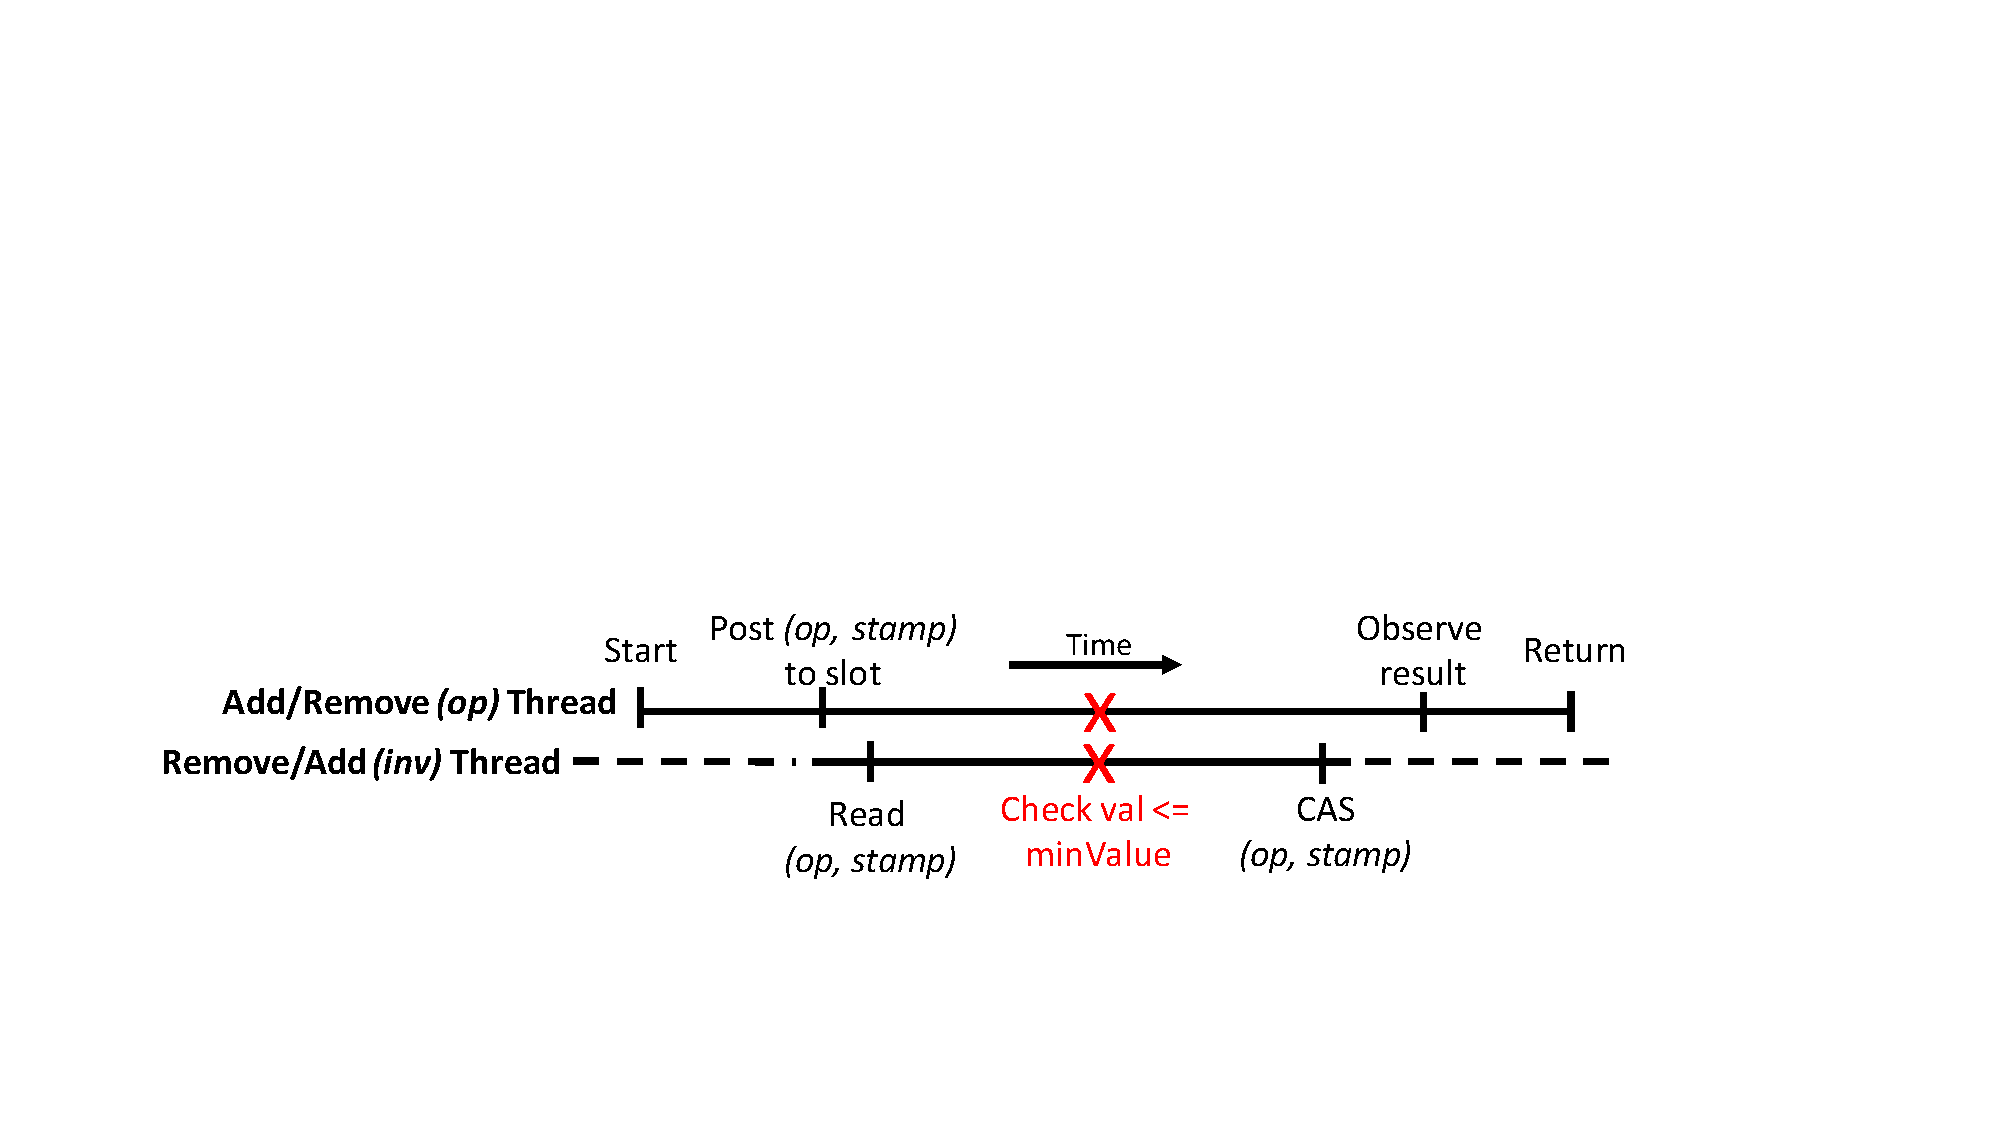
\includegraphics[width=0.9\textwidth]{graphics/correctness2.pdf}
	\caption{Execution of an \emph{op} thread and an \emph{inv} thread eliminating each others operation. The linearization point is determined through the observation of the exchanged value being smaller than \texttt{minValue}. It is marked with a red X \cite{calciu_adaptive_2014}.}
	\label{fig:correctness_elim}
\end{figure}

Figure~\ref{fig:correctness_server} shows the point in time a thread linearizes while exchanging values with the server thread. The linearizability follows from the linearizability of the skiplist itself and the sequential execution on the skiplist \cite{calciu_adaptive_2014}. 

\begin{figure}[htb]
	\centering
	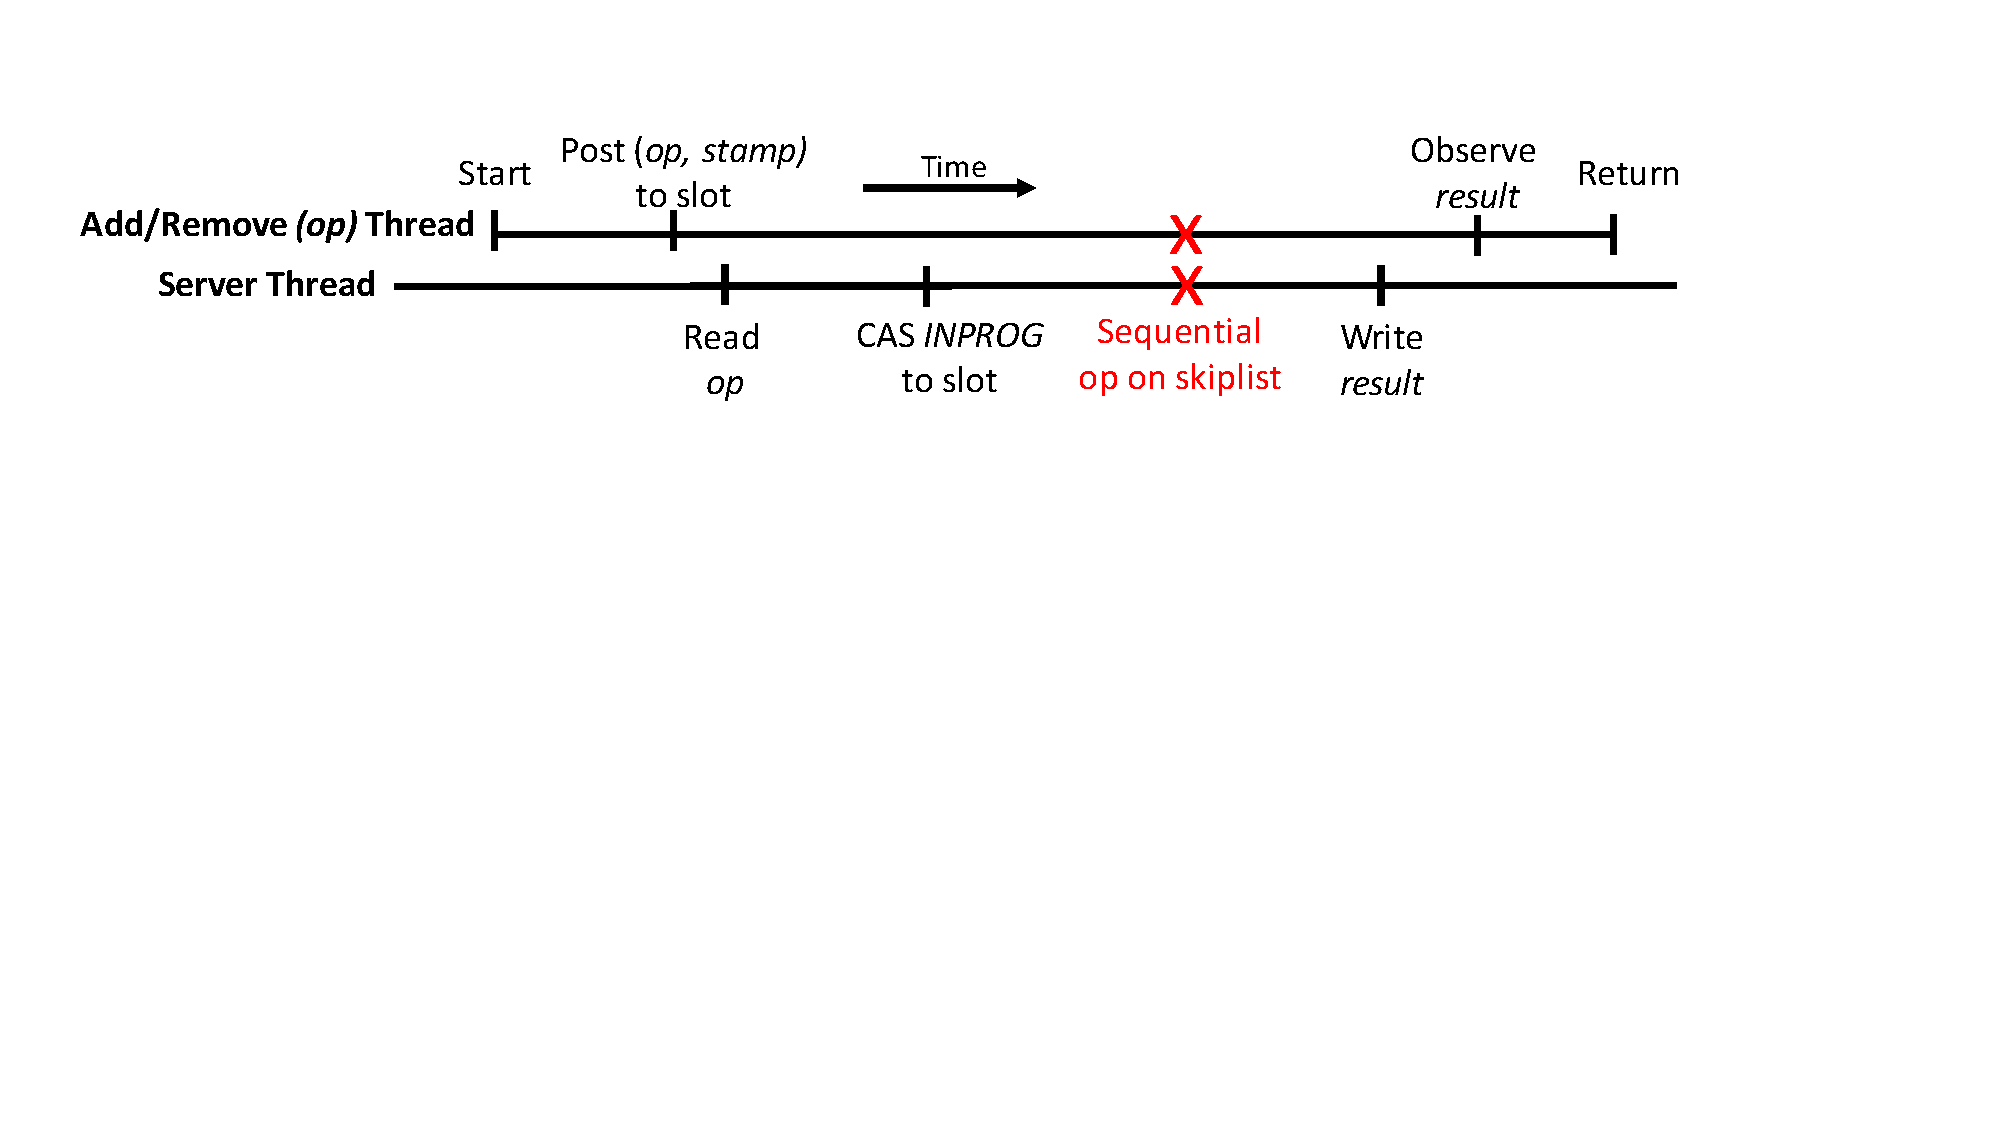
\includegraphics[width=0.9\textwidth]{graphics/correctness1.pdf}
	\caption{Execution of an \emph{op} having its operation served by the server thread. The linearization point is determined through the sequential operating server thread and is marked with a red X \cite{calciu_adaptive_2014}.}
	\label{fig:correctness_server}
\end{figure}

\subsection{Hardware Transactions}

When using transactions the linearization points are straight forward to determine. Each operation linearizes when the transaction completes successfully. 